\chapter{Methods}\label{methods}
Summarizing the key points made in \Cref{background}, current deep learning pipelines are not equipped with evaluation methods suitable for determining the degree to which predictors can generalize to \gls{ood} data, are prone to learning spurious features, and are underspecified by the datasets they are trained on. These factors can be traced back to shortcomings in \glsfirst{erm}, the theoretical basis for deep learning. The literature around developing methods to address these shortcomings tends to focus on developing more generalizable model architectures ~\cite{attention_generalizability, endocv2021_gru, doubleencdec}, data augmentation~\cite{cyclegan, polyp_augmentation, deepaugment}, Bayesian marginalization through ensembles~\cite{endocv2021_ensemble_3,divergentnets, endoensemble}, or developing novel training paradigms to directly work around the shortcomings of \gls{erm}, typically by incorporating multiple training domains~\cite{IRM, modelbased}. 

Restating the research objectives, this thesis aims both to determine the relative impacts of a number of these methods, which will be considered further in \Cref{experiments}, and to develop novel methods as informed by the theory presented in \Cref{gen_theory}, to which end this Chapter will present the following methods:

\begin{itemize}
    \item A modified DeepLabV3-based model with dual decoders, intended to constrain the space of latent representations such that underspecification is mitigated.
    \item A novel framework for analyzing generalizability based on reframing it as a predictor's ability to output predictions exhibit consistent behaviour with respect to distributional shifts, as well as a corresponding training procedure, metric and loss-function.
    \item An augmentation strategy informed by this alternative view, including both conventional augmentations and a \gls{gan}-inpainter.
    \item A family of ensemble models consisting of predictors trained according to the above methods.
\end{itemize}

This chapter will detail the development of these methods, including their basis with respect to the theory as outlined in \Cref{gen_theory}. 

\section{DD-DeepLabV3+}
As described in \Cref{background}, generalization failure can in part be attributed to the fact that most deep learning models are underspecified by the training data. In other words, the same pipeline can return any number of risk-equivalent predictors that leverage significantly different features. To mitigate this, one may impose constraints on the space of features that a given model can learn, such as through multi-task learning~\cite{ddanet}, attention-mechanisms~\cite{attention_generalizability, reverse_attention} and preprocessing~\cite{visual_cortex}. 

As testing the relative effectiveness of all of these different approaches is beyond the scope of this thesis, a simple model is instead introduced, namely a dual-decoder DeepLabV3+. As its name suggests, this model is functionally equivalent to a standard DeepLabV3+~\cite{deeplab}, but is endowed with an additional decoder, which performs image reconstruction. In theory, this should constrain the model such that it learns features that are conducive to both segmentation and reconstruction simultaneously. This constraint should mitigate underspecification and force the model to learn more generalizable features, as the feature space that is conducive to both reconstruction and segmentation naturally should be smaller than the feature space conducive to segmentation only. This does, however, presuppose that features conducive to image reconstruction also are conducive to segmentation, which may not be the case. A diagram of the model is shown in~\Cref{fig:dddeeplabv3}.
\begin{figure}[htb]
    \centering
    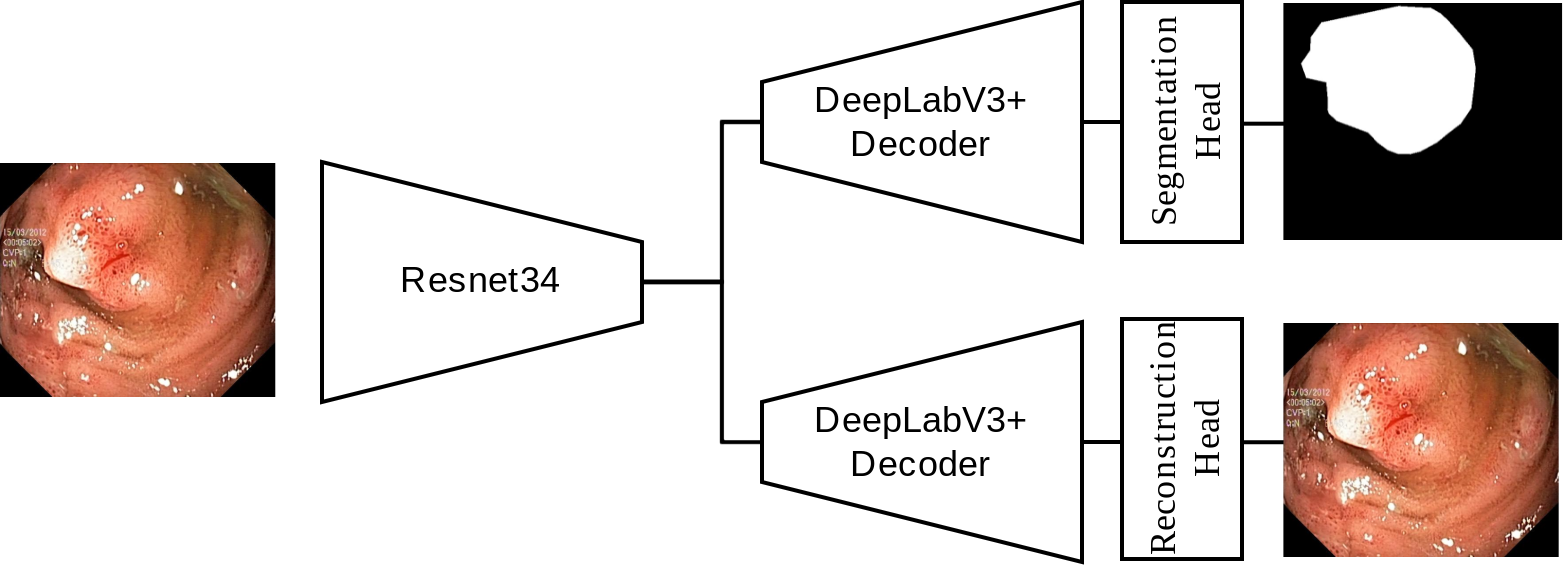
\includegraphics[width=\linewidth]{illustrations/InductiveNet.drawio.png}
    \caption[Dual Decoder DeepLabV3]{Diagram showing the Dual-decoder DeepLabV3+ model. This model uses a ResNet34 encoder to generate a feature map, which is then leveraged by two decoders concurrently. One decoder performs polyp segmentation, and the other performs image reconstruction. Functionally, the decoders are identical, and differ only in that the segmentation decoder requires sigmoid activation to map the output logits to a probability map one channel wide, whereas the reconstruction outputs the pixel values directly to three channels}
    \label{fig:dddeeplabv3}
\end{figure}

As discussed in \Cref{experiments}, this model also has the advantage of being easily compared to the standard DeepLabV3+; the part of the dual-decoder network responsible for segmentation is after all functionally identical to the single-decoder network. This facilitates better analysis of the impact of the additional decoder and its effect on the learned features, as the performance of the respective models can be compared directly. 

\section{Consistency Training}
This section will introduce Consistency Training, a training procedure wherein the objective is to optimize for invariance to a set of various image transformations by quantifying the degree to which the model outputs inconsistent predictions when its input is subjected to some transformations. This is achieved by training with two images: one which is augmented, and on which is not. The given model then performs inference on these two images, resulting in two segmentation masks. The difference between these two predictions is then computed, and compared to the difference (if any) between the augmented and unaugmented segmentation labels. This is then incorporated into the loss-function such that the discrepancy between the expected prediction change and actual prediction change is minimized. This is illustrated in~\Cref{fig:consistency_training}. The next sections will cover the theoretical basis of this training procedure as well as the implementation of its constituent components.  

\begin{figure}[htb]
    \centering
    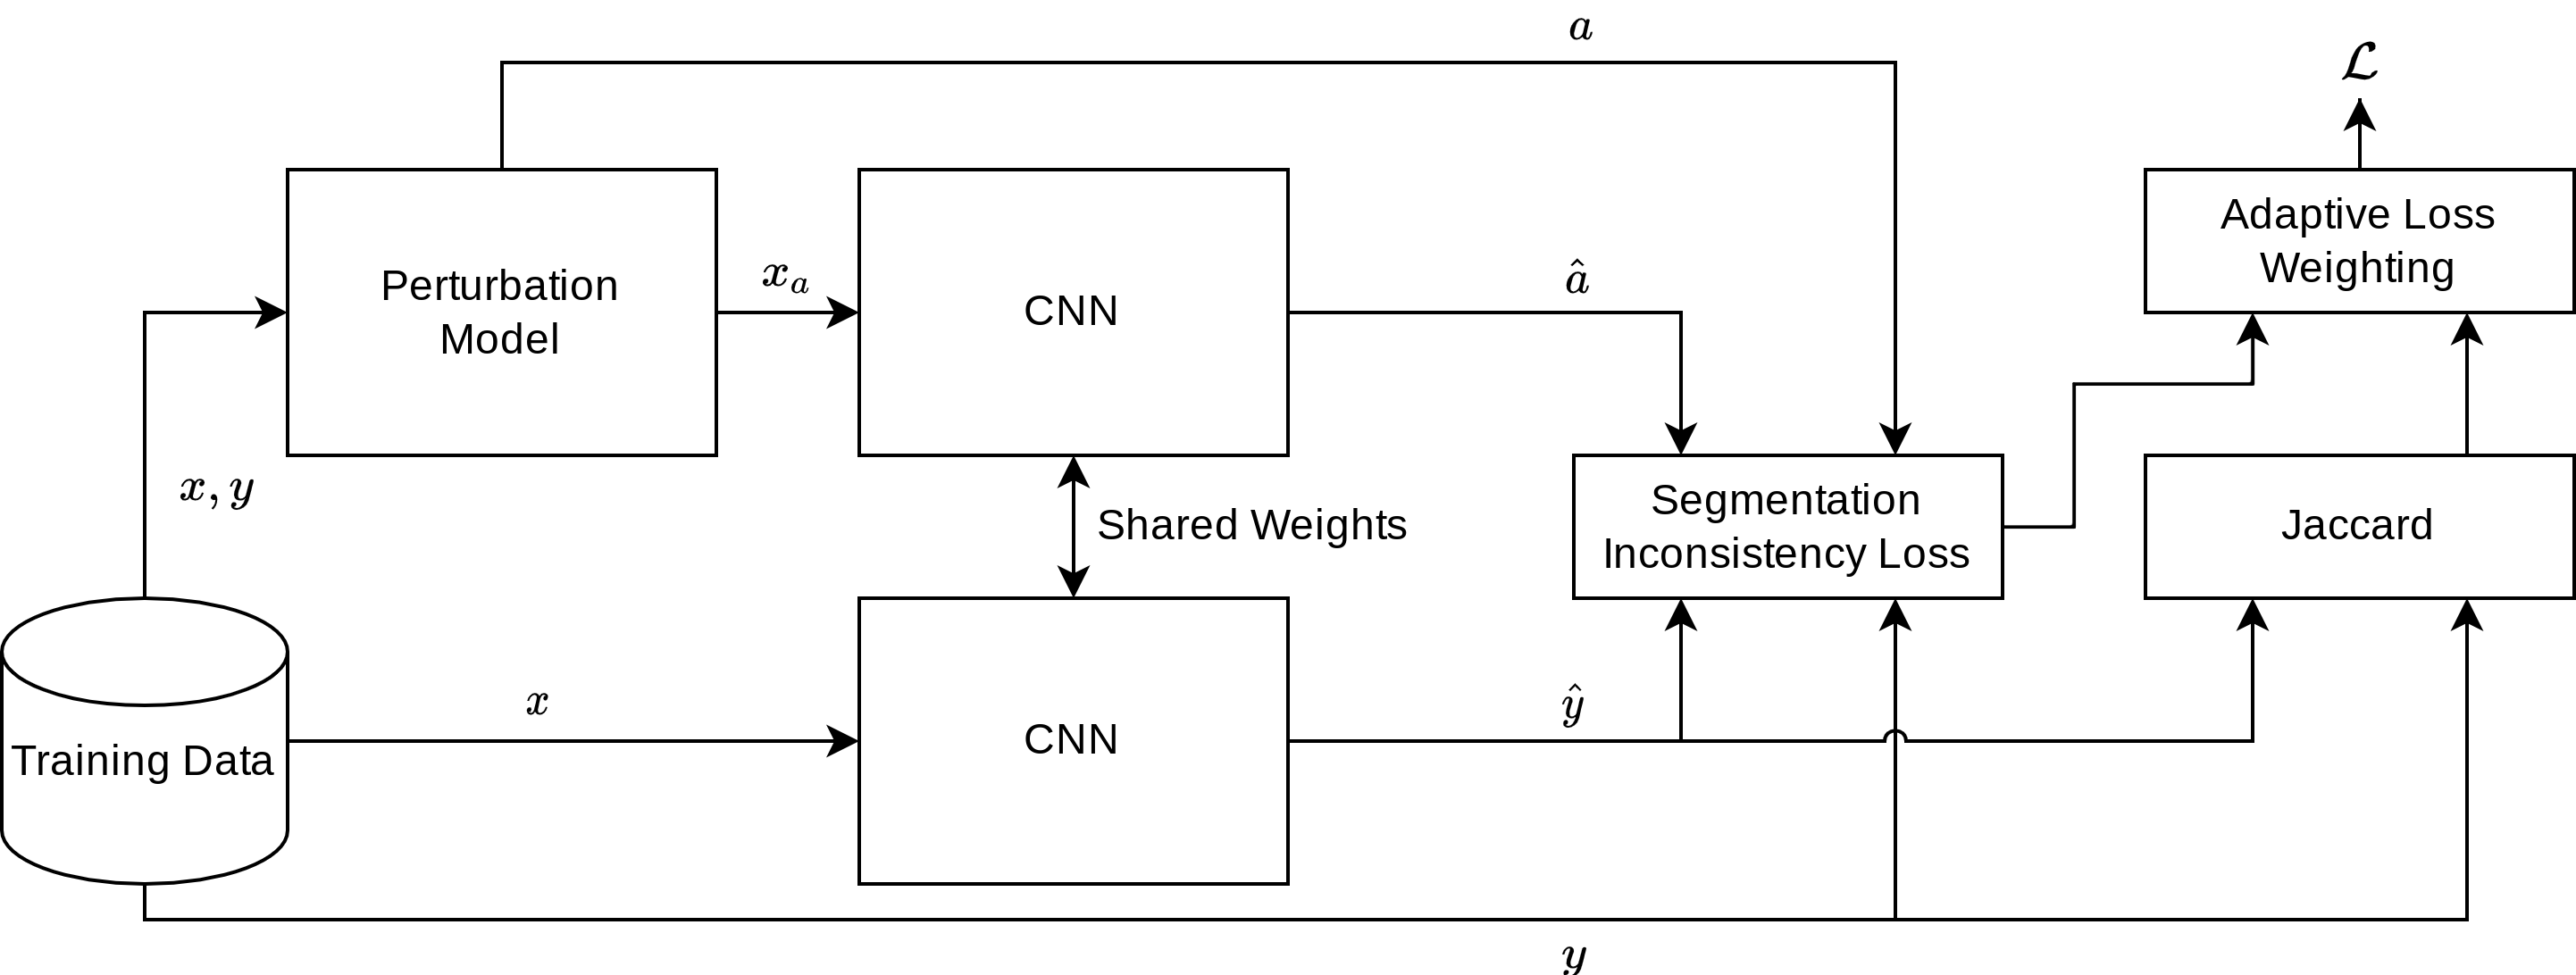
\includegraphics[width=\linewidth]{illustrations/consistency_training.png}
    \caption{Consistency Training}
    \label{fig:consistency_training}
\end{figure}


\subsection{Consistency as a Surrogate for Generalization}\label{consistency_conceptual}
As discussed in \Cref{background}, distinguishing between generalizable and non-generalizable predictors, and in turn optimizing for generalizability directly, is not feasible when evaluating only in iid-settings. This is because there is no way of knowing whether the features learned through \gls{erm} are causally related to the problem, or if they are simply predictive due to some other correlation that is strong exclusively within the bounds of the distribution given by the training data. A generalizable evaluation procedure therefore requires some way of determining whether the predictor is leveraging non-causal or causal features. 

Determining what features are causally related to the problem is, however, somewhat of an intractable problem. First and foremost, the patterns that neural networks learn and the logic that underpin them are often difficult to identify, and even more difficult to interpret on an intuitive level. Secondly, assuming there was some way of understanding these factors perfectly, establishing causality with any certainty necessitates a higher level of understanding of the problem than is reasonable to expect. 

Though establishing what \textbf{is causal} is difficult or even impossible, establishing what \textbf{is not causal} is not all that complicated. To give a concrete example, consider the problem of classifying images of cows in grassy pastures and camels in deserts. A deep learning model may just as easily learn to associate the "cow" class with grass and the "camel" class with deserts as learning what actually constitutes the respective animals. Thus, it may predict that a camel standing in a pasture or a savanna is a cow, or equivalently predict that a cow standing in a desert or on a beach is a camel. This is illustrated in~\Cref{fig:cows_and_camels}.

\begin{figure}[htb]
    \centering
    \includegraphics[width=\linewidth]{illustrations/cows_and_camels.png}
    \caption[Cows and Camels Example]{A model trained on Cows in pastures and camels in Deserts may learn to associate the cow class with grass and the camel class with sand, and thus fail to generalize even if performance on an \gls{iid} test-set is exceptional}
    \label{fig:cows_and_camels}
\end{figure}

Associating the cow class with grass and the camel class with sand is obviously non-causal, however, since this pattern would not hold if the model for instance is asked to detect cows on Mars or camels on the Moon. To mitigate this, ones first instinct may be to simply collect data of these cows and camels in a wide assortment of differing backgrounds, but such careful curation of datasets is not typically feasible, and is at any rate not guaranteed to solve the problem, as another shortcut may easily be found. In the context of polyp segmentation, is for instance not feasible to collect a dataset that is fully representative of all the differing demographics, imaging equipment, endoscopy operator faults, and so on that one may expect in deployment.  There is simply too much variation to be fully accounted for. Instead, one has to leverage the data that is actually available and try to squeeze as much utility as possible from it, either by imposing some number of a-priori inductive biases. 

Once again going back to the cows and camels example, one may for instance generate multiple instances of the same cow but with varied backgrounds and punish the model for predicting differently depending on the background. This way, the inductive bias that the predictor should be invariant to backgrounds is imposed. 

This, of course, applies to more than just modifying backgrounds: the more of these non-causal changes to the input data are accounted for and modeled, the more spurious correlations are excluded from the search, the more likely the model is to learn the patterns that are actually causal. These sorts of non-causal changes to the data will from this point on be referred to as \textit{perturbations}. These perturbations can take practically any form, only under the condition that it should not affect the causal structure of the data. If a model is trained such that invariance to all such perturbations is achieved, it must necessarily be leveraging causal features and thus be generalizable. After all, a given set of features can for all intents and purposes be considered to be causally related to the problem when the predictions generated therefrom hold when subjected to all possible perturbations. 

Thus, though rewarding causal behaviour is intractable, punishing non-causal behaviour is not. All that is required to do so is to be able to apply perturbations that highlight the non-causal reasoning the model employs, quantify the model's sensitivity to these perturbations, then minimize this quantity through optimization. The resulting model will then in theory have learned invariance to whatever causally irrelevant information that the perturbations define. This property of being invariant to perturbations will be referred to as the \textit{consistency} of the model. 

This notion of consistency can in effect be considered a surrogate for generalizability; if a model is consistent to all perturbations, it is invariant to non-causal patterns, and if it is invariant to all non-causal patterns, it necessarily employs causal patterns. Optimizing for consistency can as a result mitigate generalization failure, subject only to the span of the perturbations and how well inconsistent behaviour can be quantified.

This line of reasoning does presuppose that there is some model that can output all possible perturbations one might desire the model to be invariant to. This is of course not the case. As highlighted by the pervasiveness of adversarial attacks and the relative ineffectiveness of adversarial defenses, the perturbations that break DNNs are not necessarily intuitive, and are often difficult to analyze in a manner that is conducive to the task of engineering invariances. Nevertheless, much stands to be gained if the model learns to be invariant even to a fairly limited space of perturbations. Though generalizability is by no means guaranteed in this case, the odds of learning generalizable features are nevertheless improved simply because imposing invariance to a set perturbations limits the types of patterns that a given model can learn. If for instance a white-light endoscopic image is perturbed such that it mimics a narrow-band image, and the model learns to be invariant to this perturbation, predictors that leverage white-light or narrow-band dependent features will no longer be returned from ERM.

This approach, then, requires two components: a perturbation model, and a loss function that can describe inconsistent behaviour subject too these perturbations. One can then in turn optimize for consistency through gradient decent. The implementation of these two components will be covered in the following chapters.
    
\subsection{Implementing a Perturbation Model} \label{perturbations}
So far, it has been assumed that a perturbation model was given beforehand. This is of course not the case, and naturally any such model needs to be designed with respect to the domain in question. Rotational invariance makes sense for endoscopic images, for instance, but not for classification of hand-written numbers. Thus, in order to engineer such a model, it is first necessary to establish what invariances are desired for the given task. In the case of polyp-segmentation, it is clear that it is necessary to account for variability in for instance lighting, image-resolution, polyp-size, polyp-shape, polyp-location, camera-quality, color-shifts, blurs, optical distortions, and affine transformations. Thus, a model is required that can (more or less) parameterize this variability. Broadly speaking, these transformations can be categorized as follows:
\begin{itemize}
    \item Pixel-wise variability, which affect only the image, i.e color-shifts, brightness shifts, contrast-shifts,  blurs etc. Practically, this corresponds to changes in lighting conditions, camera motion, dye applications, etc.
    \item Geometric variability, which affect both the image and the segmentation mask, for instance affine transforms and other spatial distortions. Practically, this corresponds to endoscope orientation, optical distortion in the camera, zooming, etc. 
    \item Distributional variability, which affects both the image and the segmentation mask depending on a learned model of the distribution. Practically, this corresponds to the size, shape and location of the polyps
\end{itemize}
Pixel-wise variability and geometric variability can be modelled fairly trivially through the use of the same transformations typically used in conventional data-augmentation. Distributional variability, however, is somewhat more difficult, and requires a model that can sufficiently represent some characteristic of the distribution. This can for instance be achieved via and cross-dataset style-transfer~\cite{cyclegan, modelbased}, but this of course necessitates multiple datasets. Given only one dataset, a different method must be used. For a classification task, this could for instance be DeepAugment~\cite{deepaugment} or a similar technique. DeepAugment, however, cannot account for the changes in the segmentation mask that should be induced by the augmentations it generates. Consequently, some other generative model wherein the changes in the segmentation mask can be accounted for is required. To this end, a \gls{gan}-inpainter can be used. 

\subsubsection{GAN-based Polyp Inpainting}
As mentioned in \Cref{background}, the use of GANs and other distributional modelling in the context of generalization is typically restricted to image-to-image translation, and typically involves transforming an image drawn from one distribution such that it is \gls{iid} with a second distribution. This, though interesting and no doubt useful assuming several such datasets are available, has limited practical use. It is not necessarily always the case that there exists multiple datasets depicting identical problems, and merely translating between modalities does not as mentioned earlier in the thesis ensure generalizability.

A better approach is to try to model the training set distribution directly, then perturb the data in accordance with this model. For segmentation problems, this can be achieved through training a model to fill some predefined region with pixels that correspond to whatever segmentation target the model is meant to learn, in this case polyps, then perturb a given sample by for instance increasing the size of the polyps or adding extra polyps.

To this end, a simple GAN-inpainter was trained. The Generator \(G(\cdot)\) and Discriminator \(D(\cdot)\) were both implemented with the DeepLabV3+ architecture, and trained using the following loss formulation, where \(L_d\) and \(L_g\) corresponds to the discriminator and generator loss respectively, and \(x\) and \(y\) corresponds to masked selections of the input image and output image respectively, where the mask is given by the segmentation label. 
\begin{align}
    L_g &= 0.001 BCE(D(x),y=1) + 0.999 L1(G(x), x) \\
    L_d &= \frac{1}{2}\big[ BCE(D(G(x),y=1)+BCE(D(G(x), y=0)) \big]
\end{align}

In other words, the generator is given an image where the polyp has been masked out, and then learns to fill in the missing area. The resulting region that the inpainter fills in is then compared to the region defined by the polyp as given by the original unmasked image along with the segmentation mask, and the loss is calculated as above.

The inpainter was trained accordingly using the Adam optimizer and a cosine annealing scheduler with warm restarts. The hyperparameters are shown in~\Cref{tab:inpainting_hyperparameters}
\begin{table}[htb]
    \centering
\begin{tabularx}{\linewidth}{@{}XX@{}}
    \toprule
     Hyperparameter & Value \\
     \midrule
     batch\_size & 8 \\
     learning rate & 0.0001 \\
     epochs & 3000 \\
     Scheduler \(T_0\) & 100\\
     Scheduler \(T_{mult}\) & 2 \\
     \bottomrule
\end{tabularx}
    \caption{Hyperparameters for GAN-inpainter training}
    \label{tab:inpainting_hyperparameters}
\end{table}

Though the inpainter is trained using masks taken from the segmentation labels, inference must be done by generating a random region that is somewhat polyp-like. This was done by successively and randomly selecting points within a unit square that are a given minimum distance apart from every other point. These points were then sorted according to their order when counting counter-clockwise from the centroid, and splines generated betweem successive points between every pair of these sorted points. The region defined by this contour was then used as the inpainting target.~\Cref{fig:inpaint} shows some examples of inpainted polyps. 

\begin{figure}[!th]
    \centering
    \includegraphics[width=\linewidth]{illustrations/inpainting_examples.png} 
    \caption[GAN-inpainter rexamples]{Example outputs from GAN-inpainter, given unseen inputs taken from an unlabeled dataset. Besides certain colour artifacts, few textural details, and odd lighting, the generated polyps are moderately convincing.}
    \label{fig:inpaint}
\end{figure}


Though this implementation is by no means state-of-the-art, it should nevertheless be sufficient for the purpose of augmentation, considering the principal differences between generated and real polyp images are finer textural details and colour balancing, which are affected by the other augmentations anyway. 

\subsubsection{Geometric and pixel-wise transformations}
The data was augmented using the \textit{albumentations}~\cite{albumentations} library for python, which defines a large number of transformations for use in deep learning. To establish which of these augmentations are suitable, one first needs to establish which invariances the model(s) in question should exhibit.~\Cref{tab:vanilla_aug} below provides descriptions of the invariances required in the model, and the albumentation function that corresponds to the required transform. 
\begin{table}[htb]
    \centering
\begin{tabularx}{\textwidth}{|X|X|}
    \toprule
    \textbf{Invariance} & \textbf{Albumentation Function}\\
    \midrule
    Perspective &Flip() \newline RandomRotate90()\\
    Resolution and Zoom & RandomCrop() \\
    Image quality &GaussNoise() \newline ImageCompression()\\
    Camera models&OpticalDistortion() \\
    Lighting conditions & ColorJitter() \\
    \bottomrule
\end{tabularx}
    \caption{Overview of albumentation augmentations}
    \label{tab:vanilla_aug}
\end{table}

The parameters for the respective functions where selected as follows: one transformation was considered at a time, then parameter value(s) that still kept the polyp fairly visible but still sufficiently altered were identified. The augmentations then sample between a range given by this maximum to determine the severity for each transformation. The probability of each transformation was set to 1, such that all transformations given in~\Cref{tab:vanilla_aug} were always applied, albeit with severity being randomly selected from between 0 and the maximum as previously determined. Thus, though all the transformations were always applied, some may not have any effect if the sampled severity was close to zero. Augmentation examples without the inpainter are shown in~\Cref{fig:sample_augmentations}.

\begin{figure}
    \centering
    \includegraphics[width=\linewidth]{illustrations/augmentaion_examples.png}
    \caption{Sample Augmentations without inpainter.}
    \label{fig:sample_augmentations}
\end{figure}

It should also be noted that this set of augmentations, even including the inpainter, is of course not complete, in the sense that it accounts for all variability that one might expect in practice. As discussed previously it nevertheless may suffice to model a limited space of these transformations, as it increases the likelihood of learning generalizable features. 

Moreover, the above augmentations are not necessarily optimal, and the selected parameters are not likely to result in the best possible generalizability. In an engineering setting, the choice of augmentations should be tuned and prototyped, but for the purpose of this thesis the simple approach as outlined above is sufficient. 


\subsection{Quantifying Segmentation Consistency}

In~\Cref{consistency_conceptual}, consistency was defined as the property of exhibiting invariance to perturbations. In the context of segmentation, this corresponds to the ability of the model to output the same segmentation mask when the input data is subjected to some perturbation such as those defined in~\Cref{perturbations}.

One simple approach to express this numerically would be to count the number of pixels that do not change in the predicted segmentations when the input is perturbed, and then normalize this with respect to the total number of pixels predicted in both the perturbed and unperturbed images. This, in effect, is equivalent to calculating the \gls{iou} across the perturbed and unperturbed segmentations. However, the ground truth may of course change as a result of the perturbation - if the image is rotated, for example, the segmentation mask should be rotated accordingly. If an image is globally distorted in some way, the segmentation should exhibit the corresponding distortion. This, of course, all needs to be taken into account. This can be achieved by discounting the pixels in the predictions that are expected to change from the overall count. This quantity can be expressed as follows:

Let \(Y:=\{y,\hat{y}:=f(x)\}\) be the set consisting of the segmentation labels (masks) and predictions for the unperturbed samples, where \(f(\cdot)\) as before denotes the model. Let \(\epsilon(\cdot)\) be some perturbation function. Then, let \(A:=\{a:=\epsilon(y),\hat{a}:=f(\epsilon(x))\}\) be the set consisting of segmentation predictions and masks when the input is subjected to a perturbation. Segmentation consistency can then be quantified as:

\begin{equation}
    \mathcal{C}(A,Y) = \frac{\sum\{y \cap a \cap \hat{y} \cap \hat{a} \}}
    {\sum\{ y \cup a \cup \hat{y} \cup \hat{a} \}}
\end{equation}

A visualisation of this metric at work is shown in~\Cref{fig:consistency_example}.

\begin{figure}[htb]
    \centering
    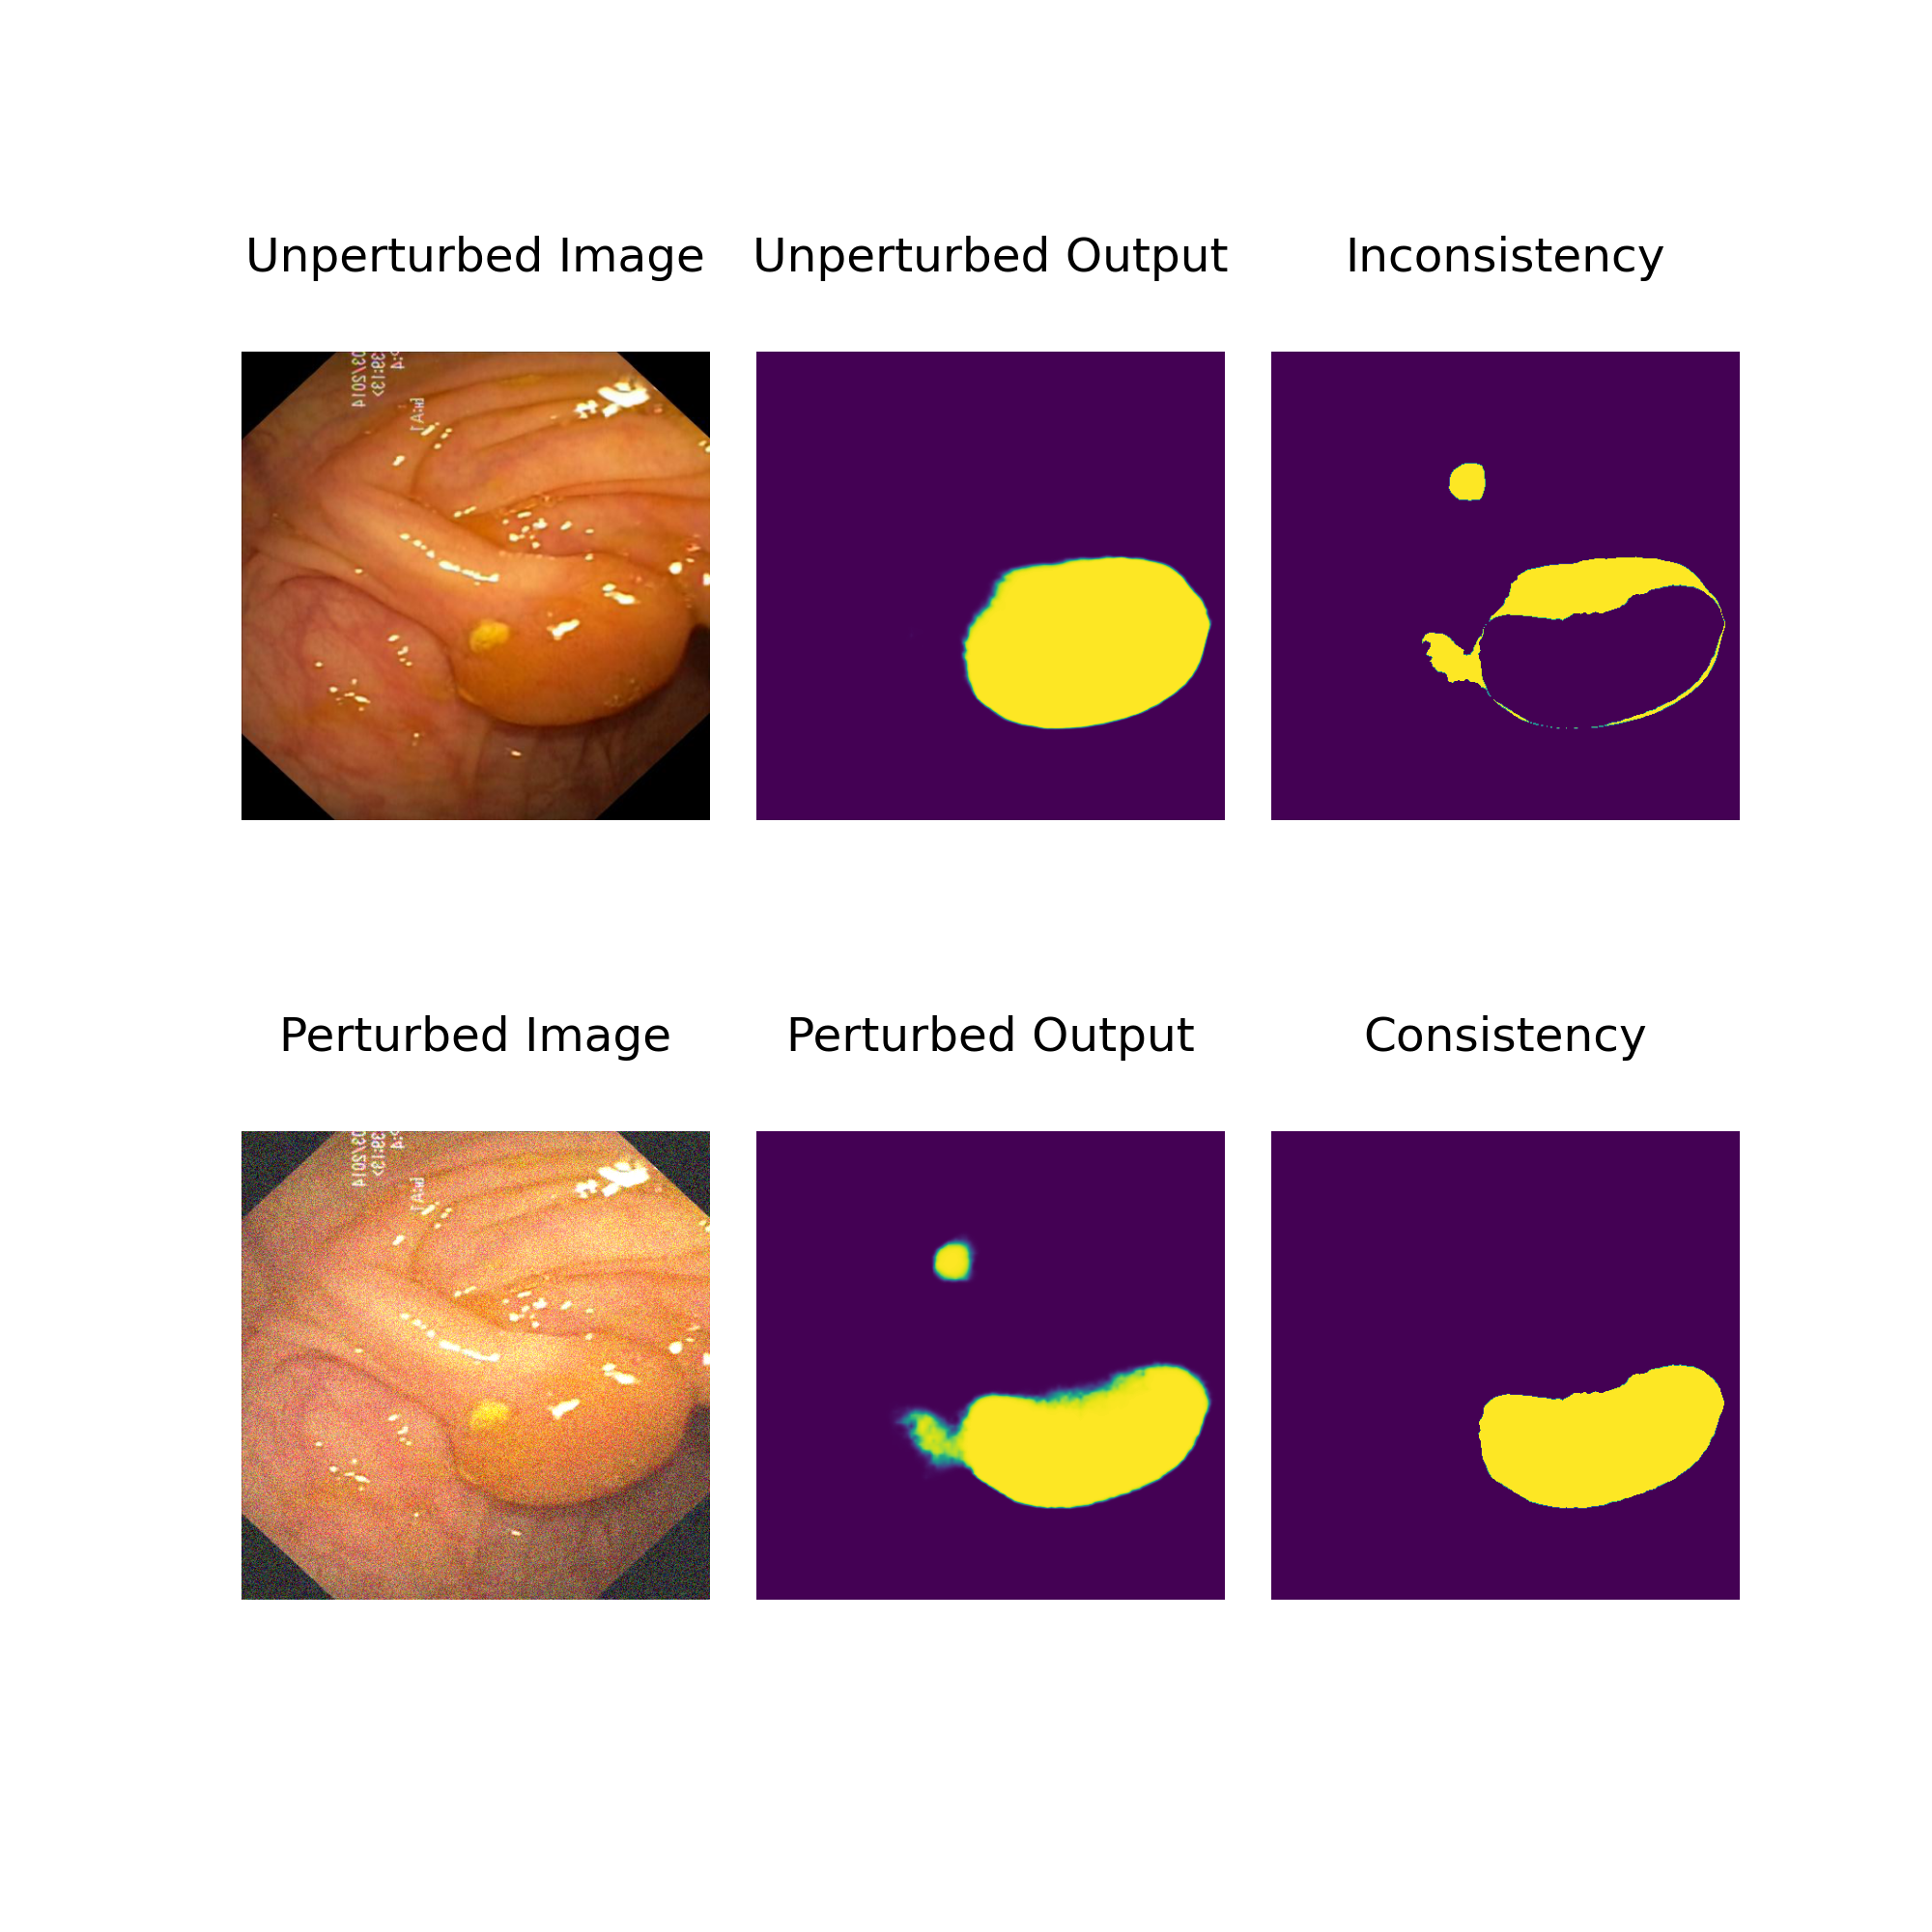
\includegraphics[width=\linewidth]{illustrations/consistency_examples.png}
    \caption[Segmentation Consistency Visualization 1]{Examples of consistency and inconsistency calculation when subjected to a non-label-altering perturbation, in this case additive noise. The consistency for this sample (when thresholded) is 0.68 and inconsistency 0.32, meaning that 64\% of the pixels constitute consistent predictions across the two inputs.}
    \label{fig:consistency_example}
\end{figure}

Using this formulation, higher is of course better. For the purpose of developing a loss function, however, it is useful to instead quantify \textit{inconsistency}. This can be expressed in much the same manner, but using the symmetric difference operator, i.e \(A \ominus B = A \cup B - A \cap B\): 
\begin{equation}\label{eq:inconsistency}
    \overline{\mathcal{C}}(A,Y) = \frac{1}{\sum\{y \cup a \cup \hat{y} \cup \hat{a} \}} \sum \{y\ominus\hat{y}\ominus a\ominus\hat{a}\}
\end{equation}
These formulations are, of course, related by:
\begin{equation*}
    \mathcal{C}(A,Y) = 1-\overline{\mathcal{C}}(A,Y)
\end{equation*}

This notion of inconsistency then corresponds to counting the number of pixels that change after the input is subjected to a perturbation - \(\hat{a}\ominus \hat{y}\), but discounting those we expect to change, \(a\ominus y\). This is also shown in ~\Cref{fig:consistency_example} and~\Cref{loss_fn}.

It is worth noting that consistency is maximized - and thus inconsistency minimized - not only if the predictions are both correct and consistent with one another, but also if the predictions are both incorrect, as long as whatever change that occurs corresponds to the expected change. This is illustrated in~\Cref{loss_fn}.
\begin{figure}[htb]
    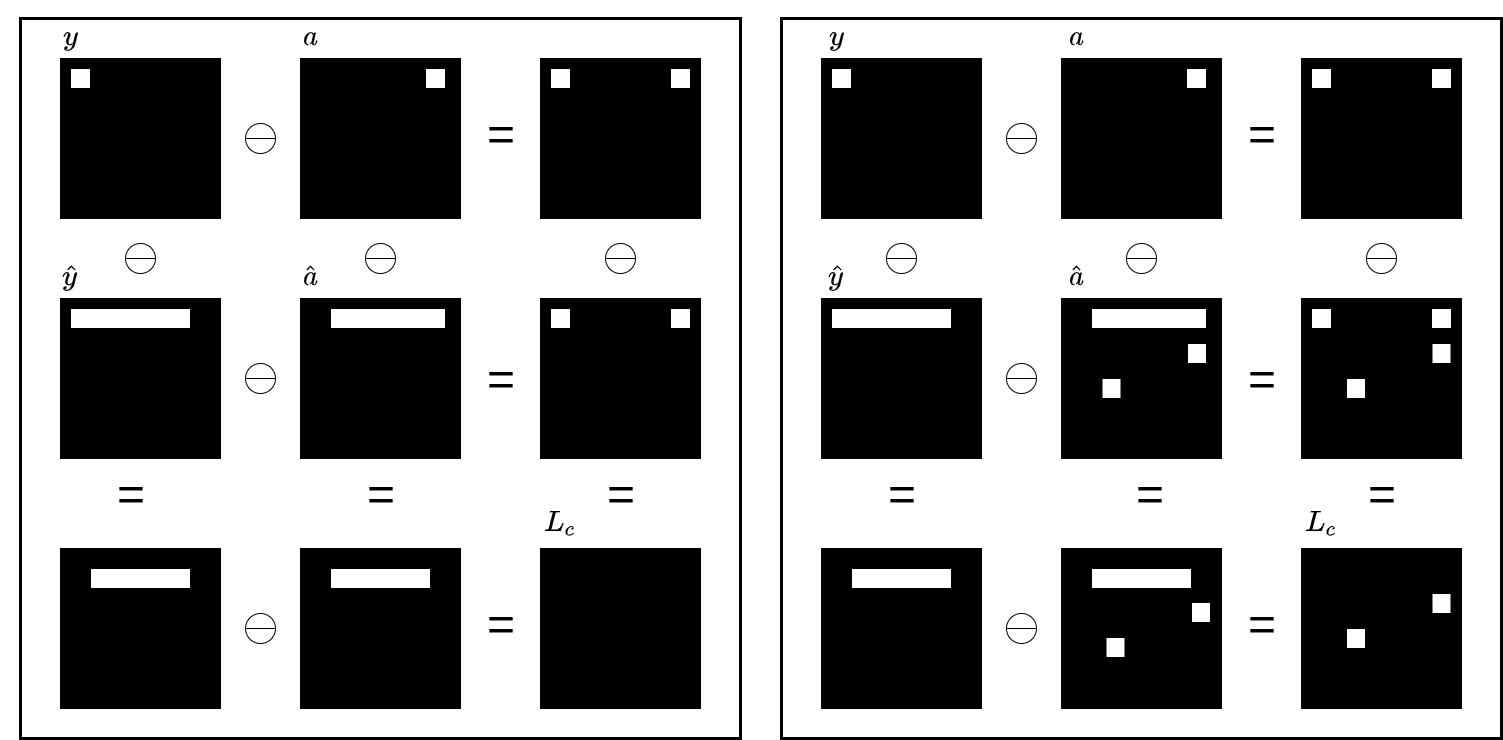
\includegraphics[width=\linewidth]{illustrations/loss_visualisation.drawio.png}
    \caption[Segmentation Consistency Visualization 2]{Visualisation of consistency calculation when subjected to a label-altering perturbation, where white is a positive prediction. Note that \(\overline{\mathcal{C}}\) is zero regardless of prediction correctness so long as it changes in the expected manner. Note also that the symmetric difference operators are associative. Left shows an instance of consistent and partially incorrect predictions, and right shows an instance of inconsistent and partially correct predictions.}
    \label{loss_fn}
\end{figure}  
    
Moreover, note that this metric does not presuppose what transformation has occurred. In~\Cref{loss_fn}, for instance, the change induced by the perturbation may correspond to simply moving the polyp in the image (and replacing the empty space with a believable background), or it may correspond to a rotation by 90 degrees. How this should be analyzed with respect to consistency is up to interpretation - one can argue that a rotation should rotate the incorrect predictions as well, or one can argue that it should only rotate the correct component of the prediction. For simplicity, Consistency Training is based on the latter interpretation. This will be discussed in further detail in~\Cref{conclusion}.

\subsection{Inconsistency Loss}
Inconsistency as expressed in~\Cref{eq:inconsistency} is not differentiable, and thus it cannot in its current state be used as a part of a loss function. This, naturally, limits the utility of the idea somewhat. Thus, a smooth extension of this metric is needed which can be achieved in much the same way as how the Jaccard loss can be derived from the Jaccard index - i.e by using differentiable versions of the set functions. 

We can extend the definition of the symmetric difference to \(\Theta(A,B) = A(1-B) + B(1-A)\). This, naturally, is equivalent to the standard symmetric difference if the values of A and B are binary. Similarly, the union operator can be extended as \( \bigcup(A,B) = A+B-AB\), and the intersection operator as \( \bigcap(A,B) = AB\). Like its binary equivalents, these operators maintain their associative and commutative properties. One can optimize for consistency by replacing the operators in~\Cref{eq:inconsistency} with these functions, which in turn can be used as a loss function:

\begin{equation}
    L_c(y, \hat{y},  a, \hat{a}) = \sum \frac{\Theta(y, \hat{y},  a, \hat{a})}{\bigcup(y, \hat{y},  a, \hat{a})}
\end{equation}

This loss function will from this point be referred to as the \gls{sil}. 

\subsection{Adaptive Loss Weighing}
    Naturally, using \gls{sil} as a loss function on its own is not really useful since it only expresses inconsistency, and is to a large extent agnostic to whatever object it is trying to segment. For instance, if the perturbation being performed is simply additive noise, the loss is equally well minimized by predicting that every pixel is positive as it is by segmenting the polyps alone. Consequently, it has to be combined with a some conventional segmentation loss, for instance Jaccard loss. A simple way to do this would be to simply add them together and normalize, i.e:
\begin{equation*}
    L(Y, A) = \frac{1}{2} \big[L_{seg}(Y)+L_c(Y,A)\big]
\end{equation*}
Preliminary experiments showed that this, however, exhibited some degree of instability. The model would readily get stuck in local minima where its predictions were indeed consistent, but also consistently predicting artifacts. Examples of this can be found in~\Cref{non_weighted_ctraining}. 

To mitigate this, it is possible to employ a weighing strategy. Instead of simply adding the respective losses together, one may weight the individual components adaptively according to the \gls{ind} segmentation performance. This way, the model will learn to predict generally correct segmentations early in the training, then start weighing consistency and as a result generalization more and more as the model sees improvements to its segmentation performance:
    \begin{equation}
        L = (1-IoU)\times L_{seg} + IoU \times L_c
    \end{equation}
Using this formulation, the model will start off trying to learn features that contribute to generally improved segmentation performance, then as segmentation performance improves start principally focusing on learning to be consistent. If the model starts veering into areas in the loss-landscape that constitute poor segmentation performance, it will self-correct by weighing the segmentation loss more. In the implementation used in this thesis, these \gls{iou} weights were calculated on a per-batch basis such that the model can quickly adapt if either of the respective objectives exhibit a degradation in performance during training. 

\subsection{Conventional Data Augmentation and Consistency Training}\label{cons_vs_aug}
    At this point, one may easily make the argument that Consistency Training is merely a somewhat more elaborate form of regular data augmentation. To some extent, this argument is well-founded; data augmentations are after all a form of perturbation, and one may argue that \gls{erm} is the mechanism by which consistency across these perturbations is minimized. There are, however, a number of nuances that separate the two methods, as will be discussed below and elaborated upon through mathematical analysis in~\Cref{discussion}. 
    
    With conventional data augmentation, one might assume that the model learns to be invariant to the augmentations as a byproduct of minimizing the empirical risk. By extension, it is assumed that the model will learn features that are equally performant across augmentations. After all, the risk-minimizing configuration is in this case that which exhibits the highest degree of performance when averaged across both augmented and non-augmented images. 
    
    This, however, is not necessarily the case. To illustrate, consider a pipeline intended to segment melanomas. As mentioned in~\Cref{gen_failure_med}, the models in such pipelines are often sensitive to skin-tone. Let us assume that the dataset consists primarily of patients with light complexions, and that data augmentation is used in an attempt to combat any bias as a result of this unbalanced dataset. For simplicity, let us assume that the only augmentation used is transforming the image with colour-jitter with probability \(p=0.5\). In theory, the empirical risk will be best minimized by learning features that do not consider colour and thus skin-tone at all, and instead simply learn to consider the shapes and sizes of the melanomas, the irregularity of which is typically considered a the principal hall-mark of melanomas. 
    
    This is unlikely for two reasons: first, it presupposes that the model readily learns these generalizable features in favor of the more predictive but spurious features during gradient decent. Second, it assumes that learning to perform well is equally easy on both the augmented and the un-augmented images. If, for instance, the model can quickly achieve high average performance and thus minimize risk locally by using color features to achieve excellent performance on the non-augmented images, while exhibiting mediocre or even poor performance on the augmented data, it is unlikely that the model will ever exit this extremely broad local minimum in favor of a more shape-biased and generalizable configuration. Moreover, it may be the case that these shape-based features require significantly more parameters in order to be able to model sufficiently and thus that the performance on the augmented data is limited to a much lower upper bound. In this case, the risk will be minimized not by learning features invariant to the transform, but by learning features that result in a sufficient equilibrium of performance across the augmented and unaugmented sets. I.e, it will try to learn predictive but brittle features as much as possible to maximize performance on unaugmented data, but under the condition that the performance does not degrade too much on the augmented data. Consistency training mitigates this by quantifying the inconsistency of the predictor subject to perturbations, and directly minimizing this quantity. Moreover, due to the weighing method used, consistency is also prioritized starting fairly early in gradient descent. 
    
    Thus, though the two methods share similar traits, they are distinct. Consistency Training can however as mentioned in~\Cref{introduction} be considered an alternative to conventional data augmentation; in pipelines wherein data augmentation is used, one can implement Consistency Training instead so long as there is a suitable method by which to quantify inconsistency. 

\subsection{Putting it all together}
To summarize, Consistency Training is based on the idea that a model necessarily must have learned generalizable features if it has learned invariance to all possible perturbations that do not affect the causal structure of the problem. This is achieved using a perturbation model \(\epsilon(\cdot)\), and a loss function which quantifies the inconsistency of the model when subjected to this perturbation. This loss term then has to be incorporated into the final loss function along with a task-specific loss, hence the adaptive loss weighing. The overall algorithm training process is shown in~\Cref{alg:consistency}:
\begin{algorithm}[htb]
    \caption{Consistency Training}\label{alg:consistency}
    \begin{algorithmic}
    \For{$epochs$}
        \For{$\left(batched\right) {x,y} \in dataset$}
        \State $x_a, a = \epsilon(x, y)$
        \State $\hat{y} \gets f(x)$
        \State $\hat{a} \gets f(x_a)$
        \State $\Bar{\mathcal{C}} \gets \frac{\Theta(\hat{x}, \hat{a},x,a)}{\bigcup(\hat{x}, \hat{a},x,a)}$
        \State $k \gets IoU(x,y)$
        \State $\mathcal{L} = (1-k) \mathcal{J}(x,y) + k \Bar{\mathcal{C}}$
        \State $f(\cdot) \gets optimizer\_update(\mathcal{L})$
        \EndFor
    \EndFor
    \end{algorithmic}
\end{algorithm}


\section{Consistency-trained Ensemble Models}
As mentioned in~\Cref{background}, ensemble-based models have demonstrated high degrees of generalizability~\cite{divergentnets, endoensemble}. Assembling predictors trained with Consistency Training into an ensemble is as a result a simple but effective means by which generalizability can be further increased. 

This can be achieved fairly simply by leveraging multiple identically trained models, such as the dual-decoder DeepLabV3+ - or indeed any model, as will be demonstrated in~\Cref{experiments}. These models can then be used to generate a unique segmentation probability map for each model. This can then be combined into a heatmap, which can then in turn be used to facilitate prediction through the use of any number of consensus methods. In this thesis, the ensembles were implemented to predict according to a simple majority-vote, i.e by thresholding the probability heatmap such that all pixels with probabilities above 0.5 were considered as positive predictions. This is illustrated in~\Cref{fig:ensemble_setup}.

\begin{figure}[htb]
    \centering
    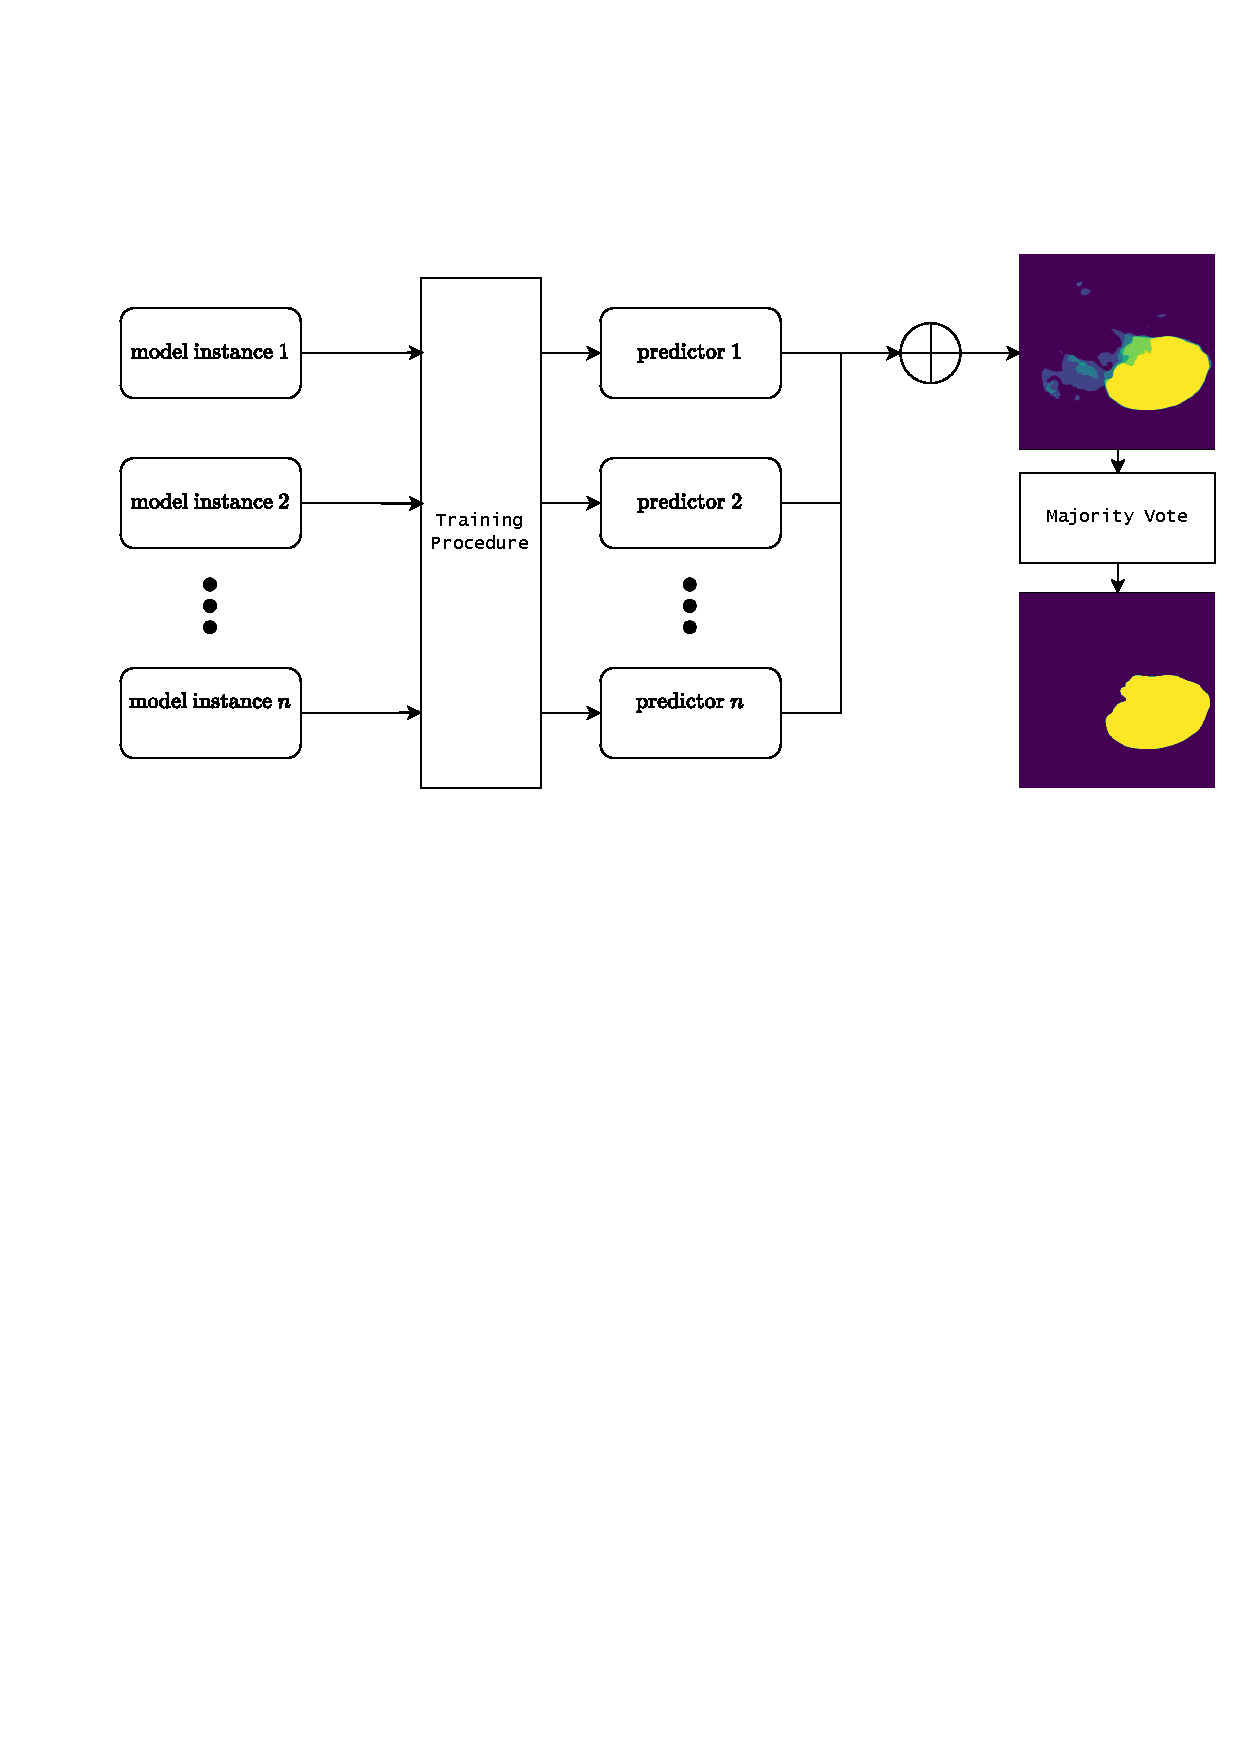
\includegraphics[trim=1.5cm 16cm 0cm 4cm, clip, width=\linewidth]{illustrations/ensemble_config.pdf}
    \caption{Implementation of Ensembles}
    \label{fig:ensemble_setup}
\end{figure}

As mentioned in~\Cref{background}, ensemble models can be considered a form of Bayesian marginalization. As a result, the model is less likely to be affected by underspecification by virtue of the fact that whatever variability in the space of features that a predictor can learn is to some extent accounted for.  

\section{Summary}
This chapter has covered the implementation and theoretical basis for the methods introduced in this thesis. The \textbf{dual decoder DeepLabV3+} aims to increase generalization by constraining the models' latent feature space through the use of image reconstruction as an auxiliary task. \textbf{Consistency training} aims to increase generalization by explicitly optimizing for consistent predictions across perturbed and un-perturbed inputs. These perturbations are application-dependent, and are in this thesis implemented as a carefully designed set of augmentations, consisting of conventional image transformations and a generative inpainting model. Finally, an \textbf{ensemble model} is implemented by combining multiple dual-decoder DeepLabV3+ models trained with Consistency Training. 